% !TEX encoding = UTF-8
% !TEX TS-program = pdflatex
% !TEX root = ../thesis.tex

%************************************************
\chapter{Hadronic Higgs Production}\label{chap:three}
%************************************************

\section{Motivation (better title needed!)}
Here I list various application for the Higgs production cross section and explain why precise predictions are so central. Maybe just put this in the chapter description?
\section{The Leading-Order Cross Section}
Having established, that the gluon-fusion Higgs production cross section is central for many phenomenological applications, we now want to perform the actual \acs{LO} calculation, which was first demonstrated by Georgi et al.\ in 1978~\cite{Georgi:1977gs}. The calculation not only serves as an instructive example on cross section calculation, and thereby allows us to put our experience from section~\ref{sec:2:cross_sections} to good use, but it already introduces many important concepts we can transfer to the \acs{NNLO} computation.

At LO, there are only two possible Feynman diagrams we can draw. They are depicted in Fig.~\ref{fig:4:LO}.
\begin{figure}[h]
\centering
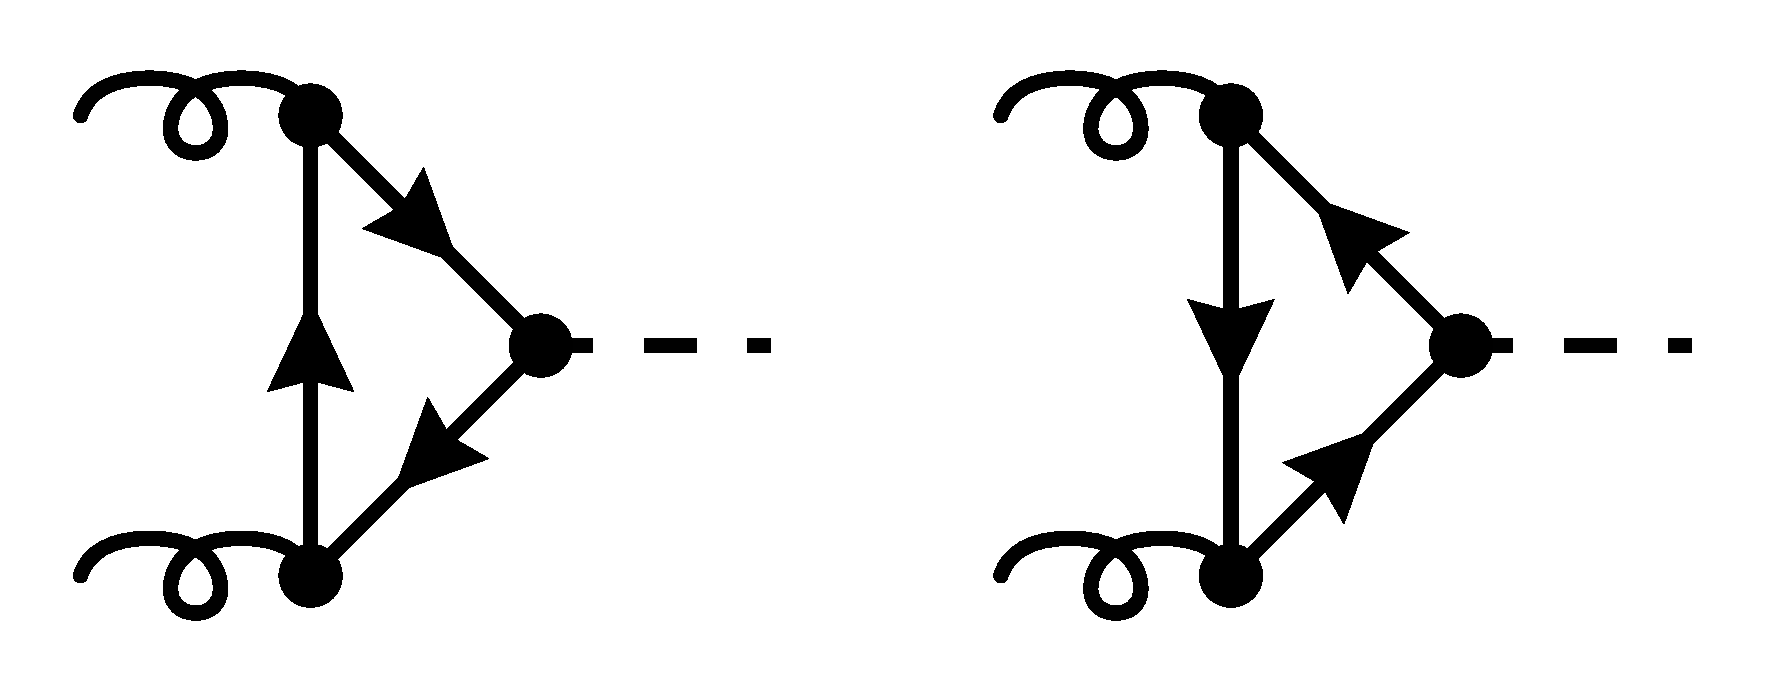
\includegraphics[scale=0.2]{Images/LO.pdf}
\caption{\acs{LO} Feynman diagrams for Higgs production in the gluon-fusion channel.}
\label{fig:4:LO}
\end{figure}
As we can see. Gluon-fusion is a loop induced process with two scales: the mass of the quark running in the loop $m_q$, and the Higgs mass $m_H$ which must simultaneously be the partonic center of mass energy. The initial state gluons carry on the on-shell momenta $p_1$ and $p_2$. Let us then define
\begin{equation}
i\mathcal{M} = i \mathcal{M}^{\mu\nu, ab} \varepsilon_\mu^a(p_1) \varepsilon_\nu^b(p_2).
\end{equation}
With the Feynman rules presented in appendix~\ref{app:1} we find
\begin{equation}
\begin{split}
&i \mathcal{M}^{\mu \nu, ab} = -\int \frac{\dd^4 k}{(2\pi)^4}\, \\
&\quad \times \text{Tr}\!\left[ \frac{-i m_q}{v} \delta_{ij} \frac{i(\slashed{k} + \slashed{p}_1 + \slashed{p}_2 + m_q)}{(k + p_1 + p_2)^2 - m_q^2} (ig \gamma^\nu T^a_{ik}) \frac{i (\slashed{k} + \slashed{p}_1 + m_q)}{(k + p_1)^2 - m_q^2} (i g \gamma^\mu T^b_{kj}) \frac{i (\slashed{k} + m_q)}{k^2 - m_q^2} \right] \\
&\quad + \lbrace p_1 \longleftrightarrow p_2,  \mu \longleftrightarrow \nu, a \longleftrightarrow b \rbrace ,
\label{eq:4:form_factor_amplitude}
\end{split}
\end{equation}
where the extra minus sign in front stems from the fermion trace.

Even without performing the explicit calculation can we already anticipate the general structure of the amplitude. Color wise, the amplitude must be proportional to $\delta^{ab}$, because it is the only available rank-two tensor. Since it is symmetric, the Lorentz structure must also be symmetric in order to satisfy \textit{Bose symmetry}. The only building blocks we have available are $g^{\mu\nu}$, $(p_1^\mu p_2^\nu + p_2^\mu p_1^\nu)$, $p_1^\mu p_1^\nu$, and $p_2^\mu p_2^\nu$, but since all transverse parts drop out of the physical amplitude, the relevant tensors are only $g^{\mu \nu}$ and $p_2^\mu p_1^\nu$. Lastly, we know that the amplitude must satisfy the \textit{Ward identity}, which allows us to restrict the tensor even further, such that we end up with
\begin{equation}
i \mathcal{M}^{\mu \nu, ab} = i\frac{\alphas}{\pi} \frac{1}{v} \delta^{ab} \left(p_2^\mu p_1^\nu - (p_1 \cdot p_2)g^{\mu\nu} \right) \mathcal{C}(m_H, m_q).
\label{eq:4:form_factor}
\end{equation}
Notice that we have only made use of very general properties of the amplitude. This is why the decomposition in Eq.~\eqref{eq:4:form_factor} will hold at every order of $\alphas$. The function $\mathcal{C}(m_H, m_q)$ is called the \textit{Higgs-gluon form factor}. It has mass dimension 2, \ie\ its functional dependence on $m_q$ and $m_H$ must be through a mass ratio
\begin{equation}
\mathcal{C} (m_H, m_q) = \mathcal{C}(z), \quad \text{with} \quad z \equiv \frac{m_H^2}{4 m_q^2}.
\end{equation}
The factor of $1/4$ was introduced, so that the \textit{normal threshold} is located at $z = 1$. Mathematically, this means that $z = 1$ is a solution of the \textit{Landau equations}, while physically, we can interpret the singularity as the point where we have enough energy to produce the quark pair on-shell. We can now project onto the form factor with
\begin{equation}
\mathcal{C}(z) = \frac{\pi v}{i \alphas} \frac{1}{N_c} \delta^{ab} \frac{1}{(p_1 \cdot p_2)^2 (d - 2)} \left(p_{2\,\mu} p_{1\,\nu} - (p_1 \cdot p_2) g_{\mu\nu} \right) i \mathcal{M}^{\mu \nu, ab}.
\end{equation}
If we now insert the \acs{LO} expression of Eq.~\eqref{eq:4:form_factor_amplitude} and perform some basic manipulations we find
\begin{equation}
\begin{split}
\mathcal{C}^{(0)} (z) = T_F \frac{1}{2 - 2 \epsilon} \frac{1}{z} \int \frac{\dd^d k}{i \pi^{d/2}} \,&\frac{1}{[k^2 - m_q^2 + i0^+][(k + p_1 + p_2)^2 - m_q^2 + i0^+]} \\
& \times \left( 2 \epsilon + \frac{m_H^2}{[(k + p_1)^2 - m_q^2 + i0^+]} \left(\frac{1}{z} + \epsilon - 1 \right) \right),
\end{split}
\end{equation}
which, after inserting integrals and expanding in $\epsilon$, finally reduces to
\begin{equation}
\mathcal{C}^{(0)}(z) = T_F \frac{1}{z} \bigg \lbrace 1 - \left(1 - \frac{1}{z} \right) \left[ \frac{1}{2} \ln\! \left( \frac{\sqrt{1 - 1/z} - 1}{\sqrt{1 - 1/z} + 1} \right) \right]^2 \bigg \rbrace.
\end{equation}
We see that the Higgs-gluon form factor is roughly proportional to the square of the mass of the quark running in the loop. One power of $m_q$ is hereby picked up from the Yukawa coupling. The factor $m_q$ is a consequence of the scalar coupling to Higgs. Indeed, without the quark mass, the trace in Eq.~\eqref{eq:4:form_factor_amplitude} would contain an odd number of gamma matrices and vanish consequently. Physically, we can interpret this as a helicity flip of the quark inside the loop, which can only occur for massive fermions. Similarly, since the two incoming gluons are vector bosons which should form a spinless final state, we would expect them to always carry opposite spins. This intuition is indeed confirmed by the tensor structure of the amplitude \eqref{eq:4:form_factor}, as it always vanishes once contracted with two polarization vectors of the same helicity\footnote{This can be seen easily by boosting to the center of mass frame and using $\epsilon^\mu (-\mathbf{p}, \lambda) \propto \epsilon^\mu (\mathbf{p}, -\lambda)$.}.

The \acs{LO} Higgs-gluon form factor is plotted in Fig.~\ref{fig:4:form_factor}.
\begin{figure}[h]
\centering
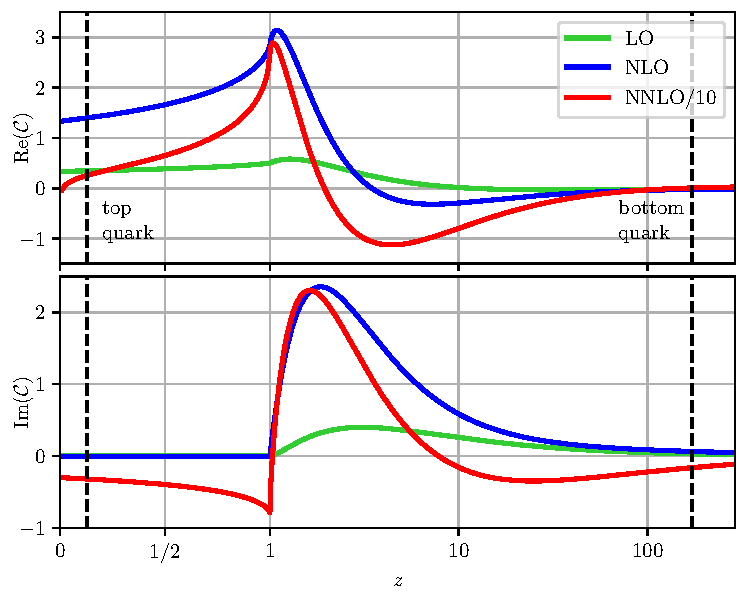
\includegraphics[width=\figurewidth]{Images/form_factor.pdf}
\caption{Real and imaginary part of the finite part of the Higgs-gluon form factor at various perturbative orders. \acs{NNLO} is divided by ten for better visibility. \acs{NNLO} results also depend on the number of light quark flavors, which has been set to 5 (5\acs{FS}). Vertical lines indicate the $z$ values for the top and bottom quark masses. The plot was created using the results of Ref.~\cite{Czakon:2020vql}.}
\label{fig:4:form_factor}
\end{figure}
As expected, we pick up an imaginary part starting from the normal threshold at $z=1$.

If we now apply Eq.~\eqref{eq:2:Xsec} and perform the phase space integration, which for a single particle is trivial because of the momentum conserving delta function, we get for the partonic cross section
\begin{equation}
\hat{\sigma}_{gg \rightarrow H} = \frac{\pi}{64 v^2} m_H^2 \left( \frac{\alphas}{\pi} \right)^2 |\mathcal{C}(z)|^2 \delta\! \left(\tau S - m_H^2 \right).
\end{equation}
The initial state was averaged over spin and color. Finally, after the convolution with the partonic luminosity we arrive at the LO cross section
\begin{equation}
\sigma_{ggH}^{\text{LO}} = \frac{\pi}{64v^2} \left(\frac{\alphas}{\pi} \right)^2 \mathcal{L}_{gg}\!\left(\frac{m_H^2}{S} \right) |\mathcal{C}^{(0)}(z)|^2.
\end{equation}
From Fig.~\ref{fig:4:form_factor} we can see that the top quark exerts the largest impact on the Higgs-gluon form factor and hence the \acs{LO} hadron cross section. We can read off the partonic luminosity from Fig.~\ref{fig:2:luminosity} and find that the cross section for the top quark induces Higgs production reads\footnote{Values of masses and coupling constants are provided in the \hyperref[chap:notation_and_conventions]{conventions}.}
\begin{equation}
\sigma_{ggH}^{\text{LO}} (t) = 16.30\ \GeV
\end{equation}
at a hadronic center of mass energy of $13\ \text{TeV}$. Although expected to have little impact, we can also include the effects of finite bottom quark masses by coherently summing together the corresponding form factors. We find
\begin{equation}
\sigma_{ggH}^{\text{LO}}(t+b) = 14.72\ \GeV,
\end{equation}
\ie\ the bottom quark lowers the cross section by around $9\%$ at \acs{LO}.

Without the inclusion of electro-weak corrections, we can always decompose the gluon fusion cross section in terms of the Yukawa couplings $Y_i$:
\begin{equation}
\sigma_{ggH} =  \sum_{i\le j} Y_i Y_j \sigma_{i j}.
\end{equation}
We call
\begin{equation}
\sigma_{i \times j} = Y_i Y_j \sigma_{ij},
\end{equation}
the \textit{i-j-interference contribution} and
\begin{equation}
\sigma_{i} = Y_i^2 \sigma_{ii}
\end{equation}
the \textit{pure-i contribution} to the cross section. Both contributions are depicted at \acs{LO} in Fig.~\ref{fig:4:quark_effects}.
\begin{figure}[h]
\centering
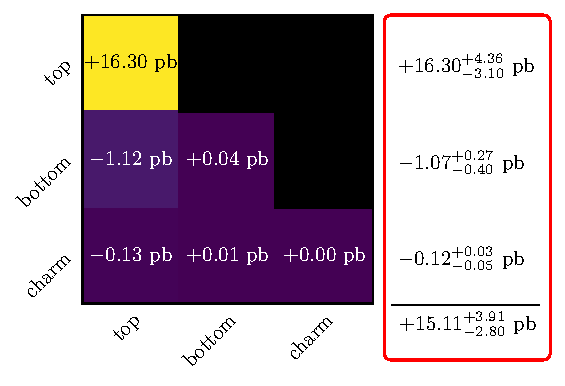
\includegraphics[scale=1]{Images/quark_effects_LO.pdf}
\caption{$\sigma_{i}$ (diagonals) and $\sigma_{i \times j}$ (off-diagonals) at \acs{LO} for the three heaviest quark flavors. The red box indicates the sum of each row, and hence the combined effects of each additional flavor. Computational setup is described in the \hyperref[chap:notation_and_conventions]{conventions}}
\label{fig:4:quark_effects}
\end{figure}


\section{The Heavy-Top Limit}
Here I explain the heavy-top limit.
\section{Higher-Order Corrections}
Here I outline how to perform higher order corrections.
\section{Theory Status}
Here I describe what is already known about the gluon-gluon fusion channel. I explain the theory uncertainties.

